\begin{comment}
	\pagebreak
\end{comment}

\section{Neural Implicit Representations}
\textbf{Traditional:} cam, pointcloud, mesh, tracked mesh\\

\textbf{Voxel:} 3D grid, limited resolution in $O(n^3)$\\
\begin{comment}
	If we use a signed distance Field, it has similar properties.\\
\end{comment}

\textbf{Points:} Sensor meassurements, no connectivity/ topology\\

\textbf{Mesh:} Vertices and surfaces, -self-intersections, -discont.\\
\begin{comment}
	A big differentiation can be made between implicit and explicit surfaces.
	A mesh is explicitely defining vertices and surfaces, which introduces an approximation error, since only a finite amount of elements are used.
	With an implicit function, we can check wheater a point is on the surface really cheap and quick.\\
\end{comment}

\textbf{Implicit Repr.:} set-level of cont. function, +no approx error, +combining, +exact, -intersection comput and exact\\
store SDF values on a regular grid\\
\textbf{Neural Impl. Repr:} function as NN represents shape; +low memory\\
\begin{comment}
	This achieves arbitrary topologies and resolutions, the function is also continous.
	We remove the memory bottleneck like this.\\
	
	What we want is a function that inputed a location, gives us a distance meassure:
	\begin{Figure}
 		\centering
 		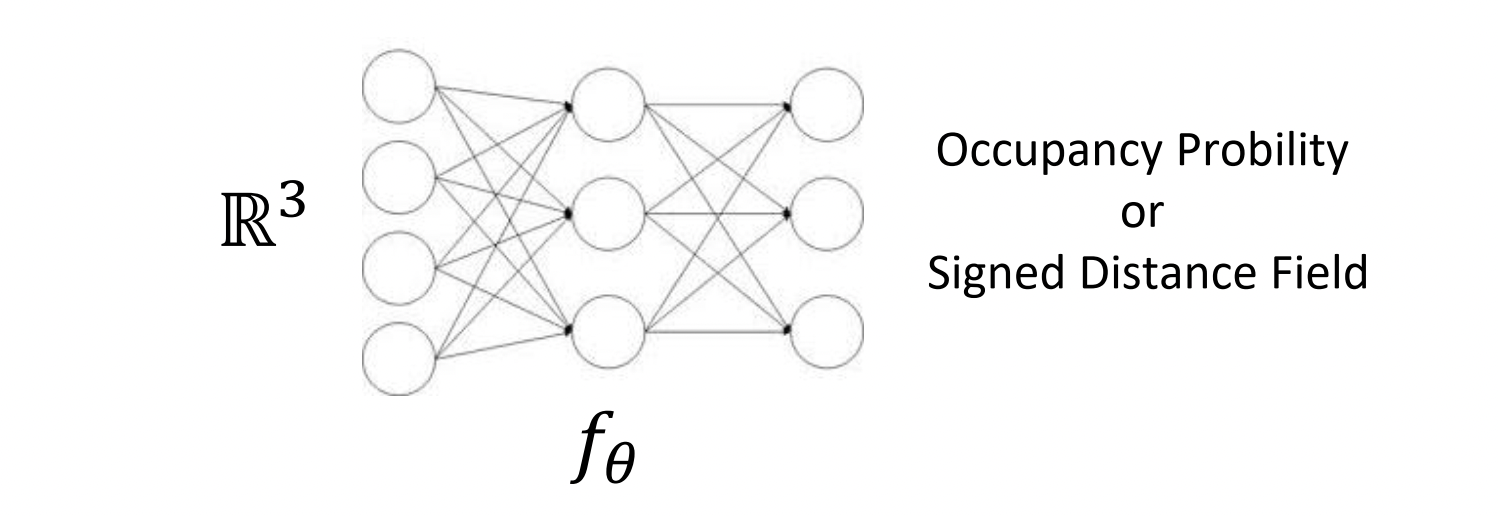
\includegraphics[width=\linewidth]{graphic/nir-implementation}
 		\captionof{figure}{NIR representation}
	\end{Figure}
\end{comment}

% with 3D supervision
\textbf{from Mesh:} $\cL(\theta, \phi) = \sum BCE(f_\theta(p_{ij}, z_i), o_{ij})$, rand. query\\
\begin{comment}
	p is position, o is occupacy.
	The MLP learns decision boundary, which concides with inside and outside the mesh here.\\
\end{comment}

\textbf{from Pointcloud:} $\cL(\theta) = \sum |f_\theta(x_i)|^2 + \lambda \E_X(\norm{\nabla_X f_\theta(x)} - 1)^2$\\
\begin{comment}
	The Eikonal function (shortest path'ish) with wave velocity 1 is converging to the signed distance function when used with MLP.
	\Note{Much harder than from Mesh, since only (noisy) point of the surface to create boundary}\\
\end{comment}

\textbf{Eikonal PDE:} $\norm{\nabla f(x)} = 1, f(x) = 0, x \in \Omega$, gives SDF $\Omega$\\
$\cL(\theta) = \Sigma_i \abs{f_\theta(x_i)}^2 + \lambda \E_X(\norm{\nabla_x f_\theta(x)} - 1)^2$; converges!\\


% without 3D supervision
\textbf{Derivating Volume rendering} point location + encoded picture, 5 ResNet, Occupancy and Texture head\\
\begin{comment}
	Occupancy meassures if we are on the surface, behind or in front of the surface.
	
	\begin{Figure}
 		\centering
 		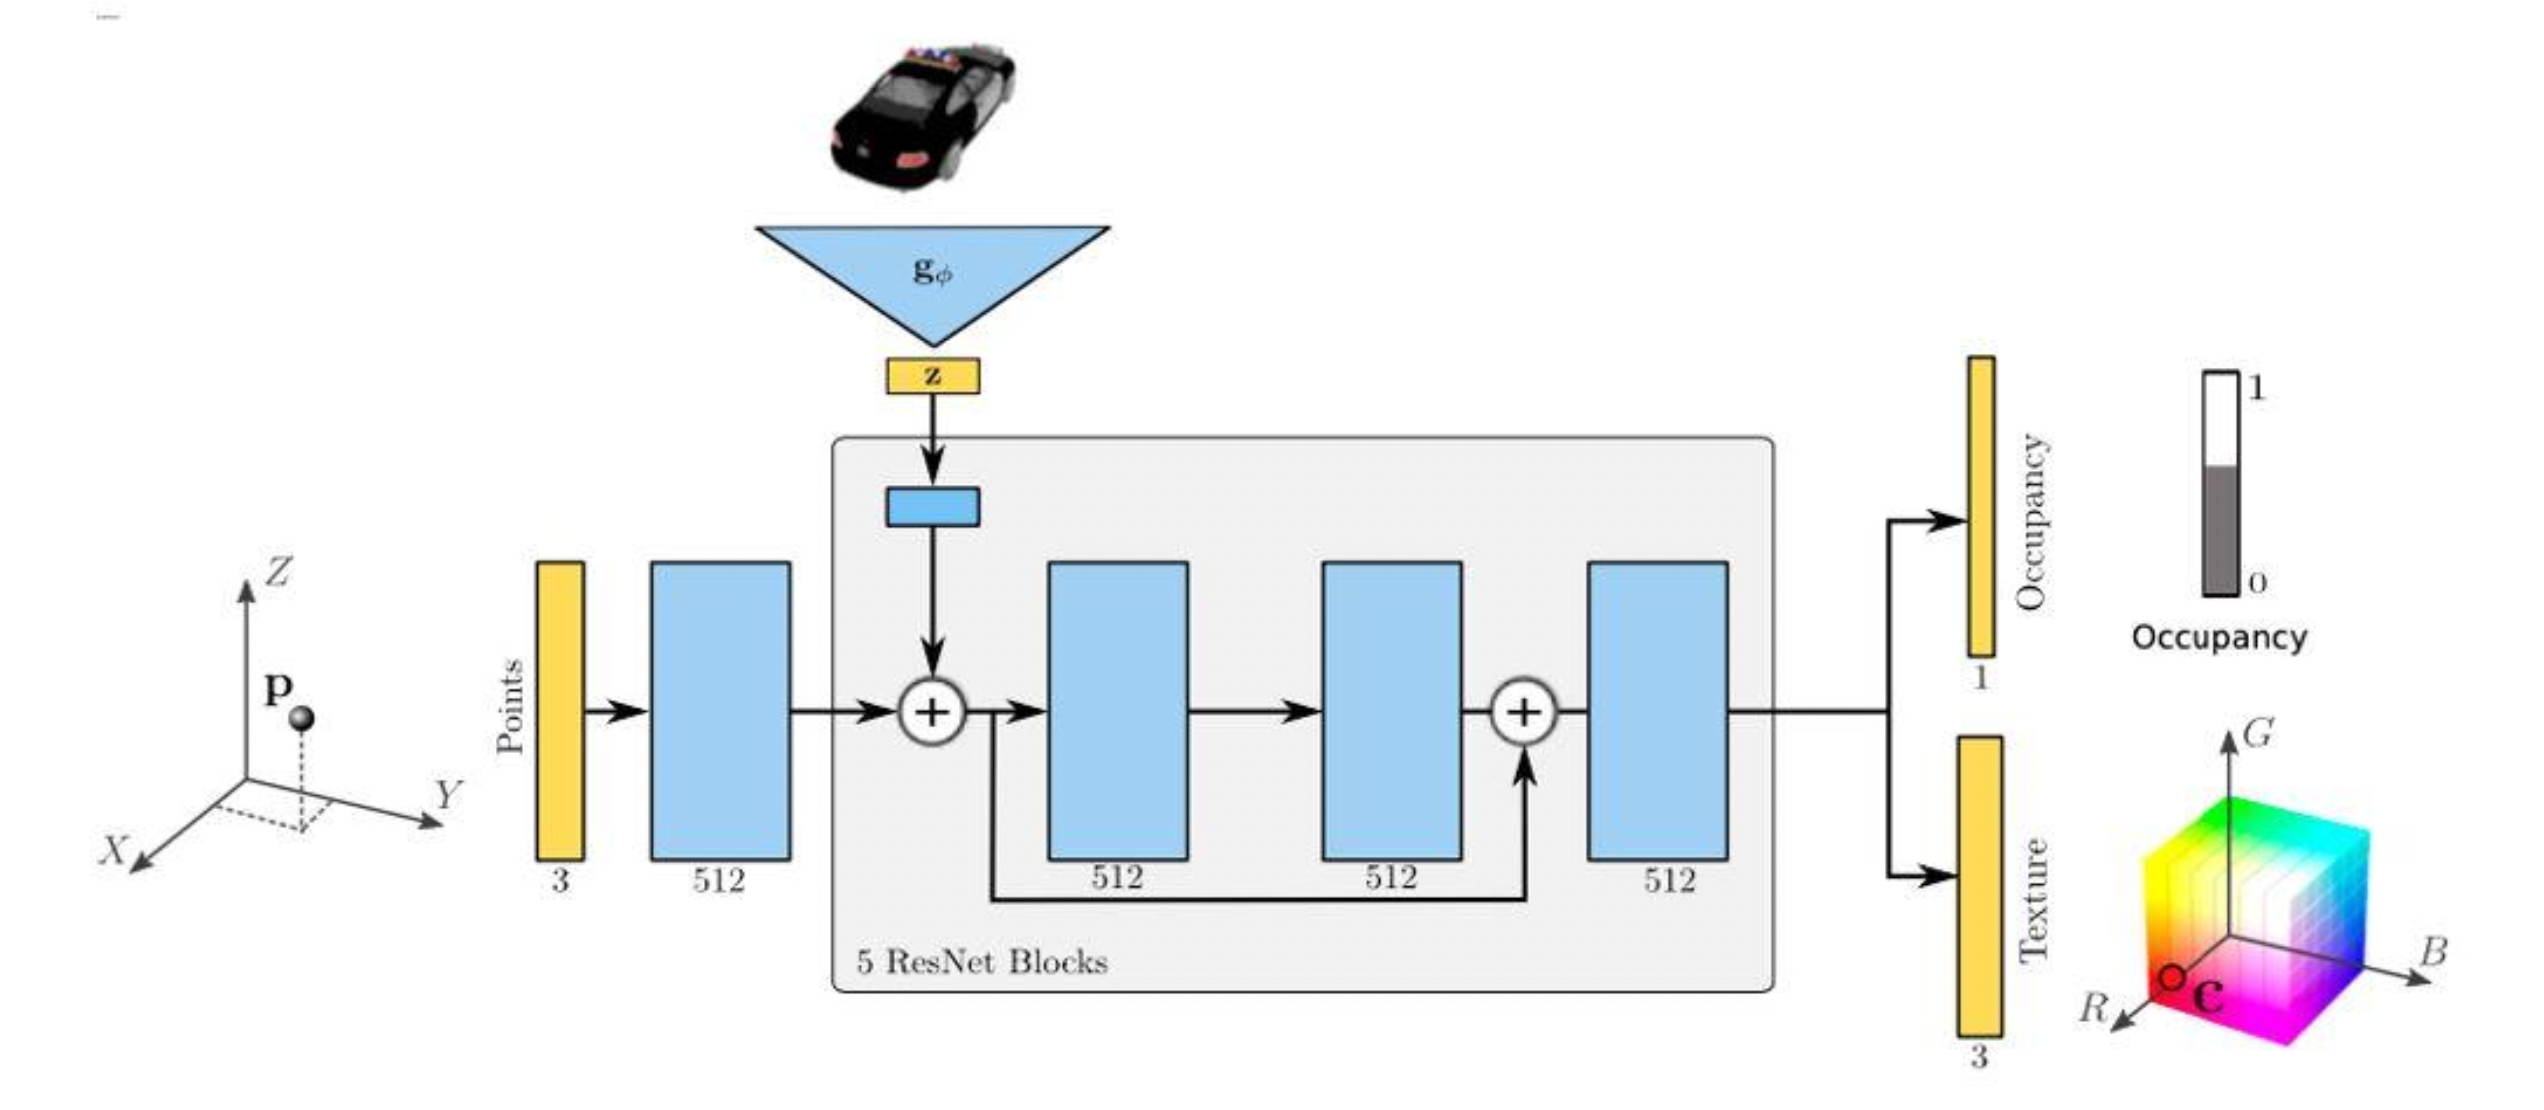
\includegraphics[width=\linewidth]{graphic/nir-dvr}
 		\captionof{figure}{NIR Derivating Volume rendering}
	\end{Figure}
\end{comment}

\textbf{Forward:} $\forall u$, ray from $r_0$ through $u$ to root $\whp$ ($\downarrow$), $u = t_\theta(\whp)$\\
$y_2 = \frac{f(x_1) - f(x_0)}{x_1 - x_0}(x_2 - x_1) + f(x_1), x_2 = x_1 - f(x_1) \frac{x_1 - x_0}{f(x_1) - f(x_0)}$\\

\textbf{Render:} shoot rays, rough occupancy est., secant, texture query\\
\begin{comment}
	We assume to know the camera position, from there we shoot rays though the pixels of the image and query occupancy for equidistant points.
	Query the color for the intersection point from the texture head.\\
	
	\begin{Figure}
 		\centering
 		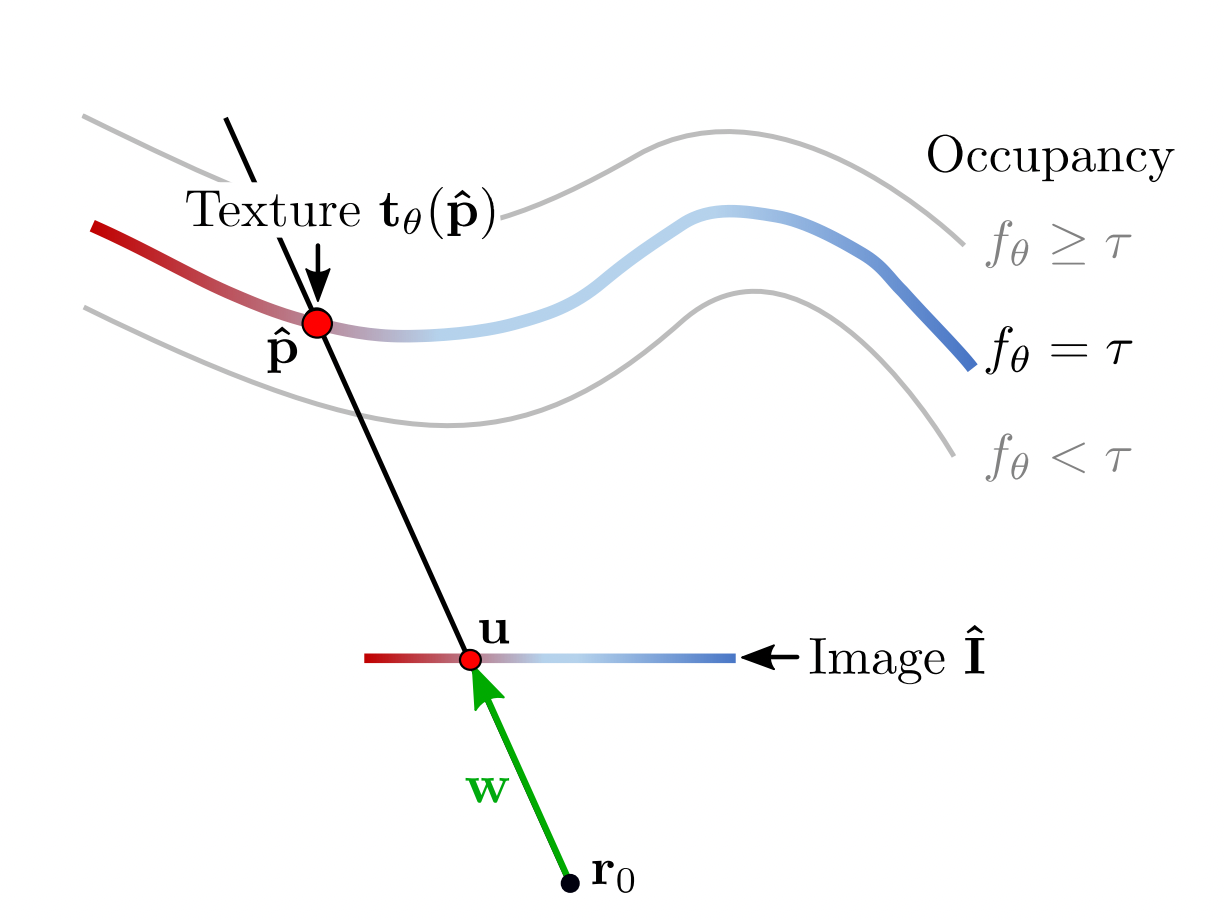
\includegraphics[width=\linewidth]{graphic/nir-dvr-forward}
 		\captionof{figure}{NIR DVR forward pass}
	\end{Figure}
\end{comment}

\textbf{Backprob:} $\cL(\whI, I) = \sum \norm{\whI_u - I_u}$, $\frac{\partial \cL}{\partial \theta} = \sum \frac{\partial \cL}{\partial \whI_u} (\frac{\partial t_\theta (\whp)}{\partial \theta} + \frac{\partial t_\theta(\whp)}{\partial \whp} \frac{\partial \whp}{\partial \theta})$,
$\frac{\partial \whp}{\partial \theta} = -w(\frac{\partial f_\theta(\whp)}{\partial \whp} w)^{-1} \frac{\partial f_\theta(\whp)}{\partial \theta}$\\



\textbf{NeRF:} $F(x,y,z, \theta, \phi) \rightarrow (r,g,b,\sigma)$, whereas F is FCNN w. ReLU\\
-static only, -slow render, -need many views\\
\begin{comment}
	Each MLP is overfitted to one object/scene it was trained on, it really is a composition of multiple views.\\
	Input is (x,y,z) and viewing angle ($\theta, \phi$); output is color and density.
	Transparency is only dependend on location, color is dependend on both (reflection).
	The viewing direction is only fed into the network really late, which allows to focus on geometry and only finetune the view dependend color.
	
	\begin{Figure}
 		\centering
 		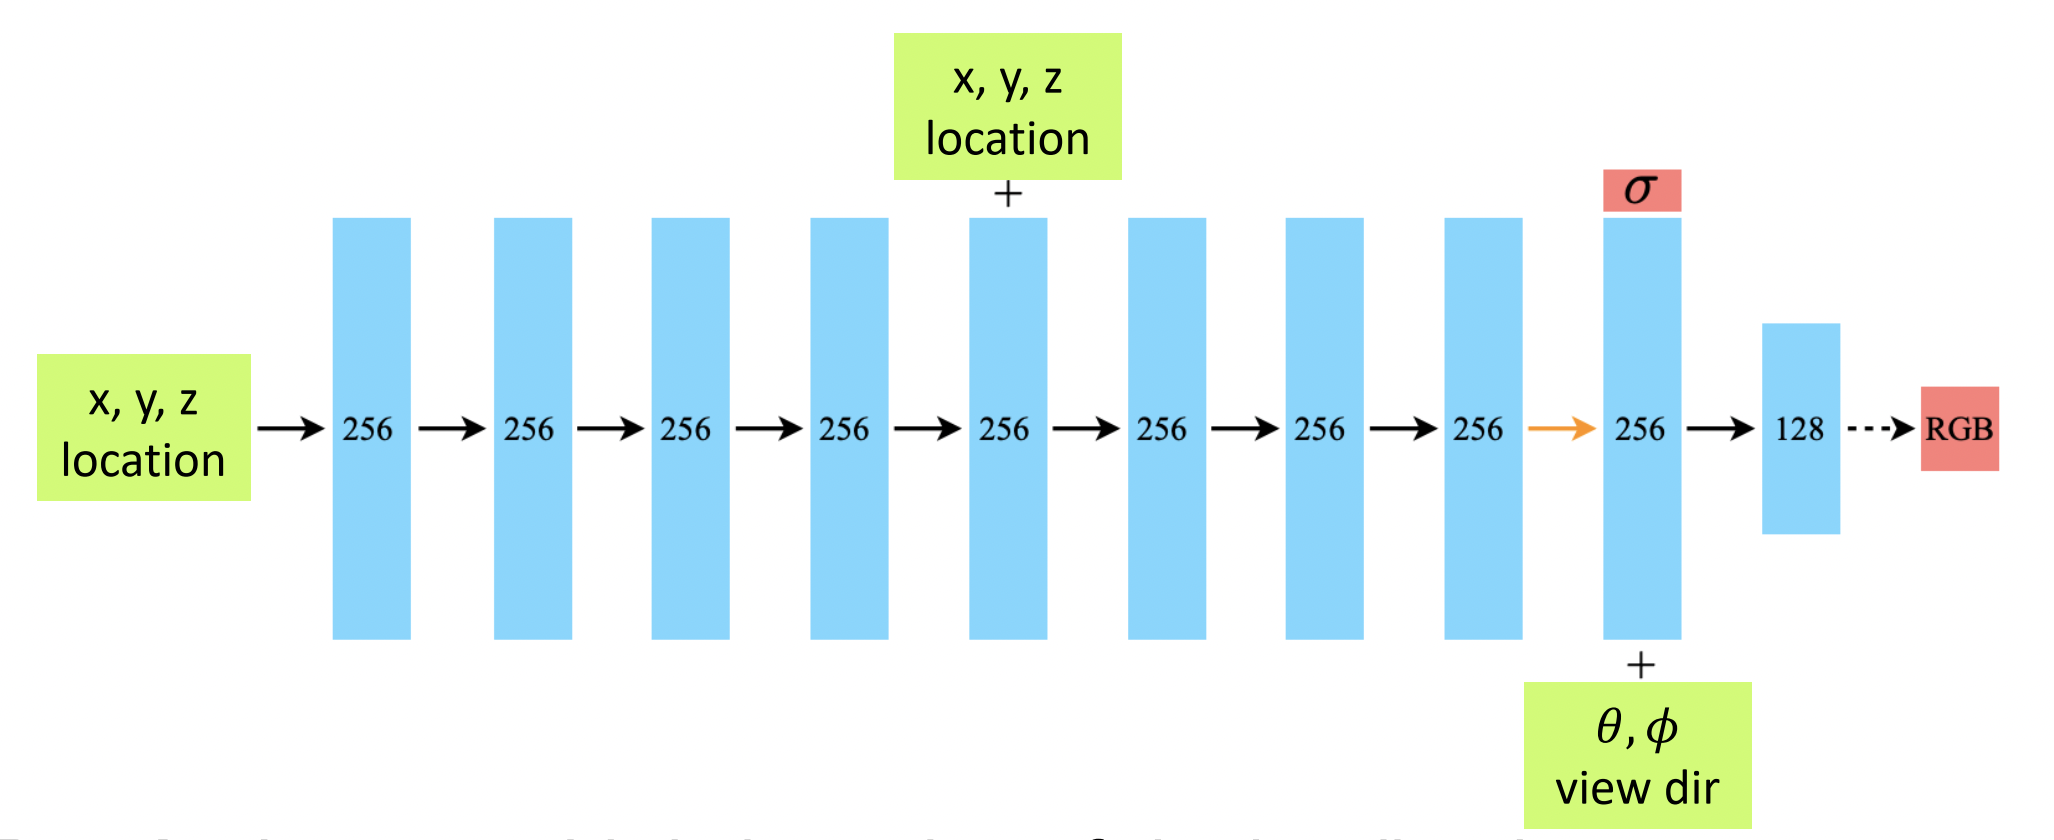
\includegraphics[width=\linewidth]{graphic/nir-nerf-architecture}
 		\captionof{figure}{NIR NeRF Architecture}
	\end{Figure}
\end{comment}

\textbf{Render:} Shoot ray, evaluate all, alpha compose for color\\

\textbf{$\alpha$-composition:} $\alpha_i = 1- e^{-\sigma_i (t_{i+1} - t_i)}$\\
\textbf{Transmittance:} $T_i = \prod_1^{i-1} (1-\alpha_j)$, 
\textbf{Color:} $c = \sum T_i \alpha_i c_i$\\
\begin{comment}
	Alpha is saying if at a certain point is something that emits light ($\sigma$), multiplied by a scaling factor.
	The transmittance is modelling the impact of color down the ray.\\
\end{comment}

\textbf{Positional encoding:} location in fourier space, easier to approximate high frequencies\\



